\documentclass{article}
\usepackage{tikz}
\usetikzlibrary{tikzmark,calc}

\newcommand{\riquadro}[1]{%
\tikz[remember picture,overlay]
 \draw[line width=1pt,rectangle,rounded corners,fill=blue!10,draw=blue]
  (pic cs:#1) ++(0.05,-0.15) rectangle (0.05,0.35);
}
\thispagestyle{empty}
\begin{document}

\riquadro{a}Testo da evidenziare\tikzmark{a}\\[2ex]
\begin{tikzpicture}[remember picture,overlay]
\draw[red] plot[mark=x]  coordinates{(pic cs:a)} node[right]{\scriptsize{\texttt{pic cs:a}}};

\draw[brown!50!black] plot[mark=x]  coordinates{($(pic cs:a)+(0.05,-0.15)$)} node[below]{\scriptsize{\texttt{(0.05,-0.15)}}};

\draw[brown!50!black] plot[mark=x]  coordinates{($(pic cs:a)+(-3.225,0.35)$)} node[left]{\scriptsize{\texttt{(0.05,0.35)}}};
\end{tikzpicture}
\end{document}